\documentclass[tikz,border=8pt]{standalone}
\usepackage[utf8]{inputenc}
\usepackage[T1]{fontenc}
\usepackage{lmodern}
\usetikzlibrary{arrows.meta,positioning,fit}
\definecolor{navy}{HTML}{15324B}
\definecolor{blue}{HTML}{2F80C1}
\definecolor{cyan}{HTML}{DCEFF7}
\definecolor{orange}{HTML}{E8873A}
\definecolor{green}{HTML}{3B8F72}
\tikzset{box/.style={draw=navy,rounded corners=3pt,very thick,align=center,minimum width=2.7cm,minimum height=1.15cm,fill=white,font=\sffamily},arr/.style={-{Latex[length=3mm]},very thick,navy}}
\begin{document}
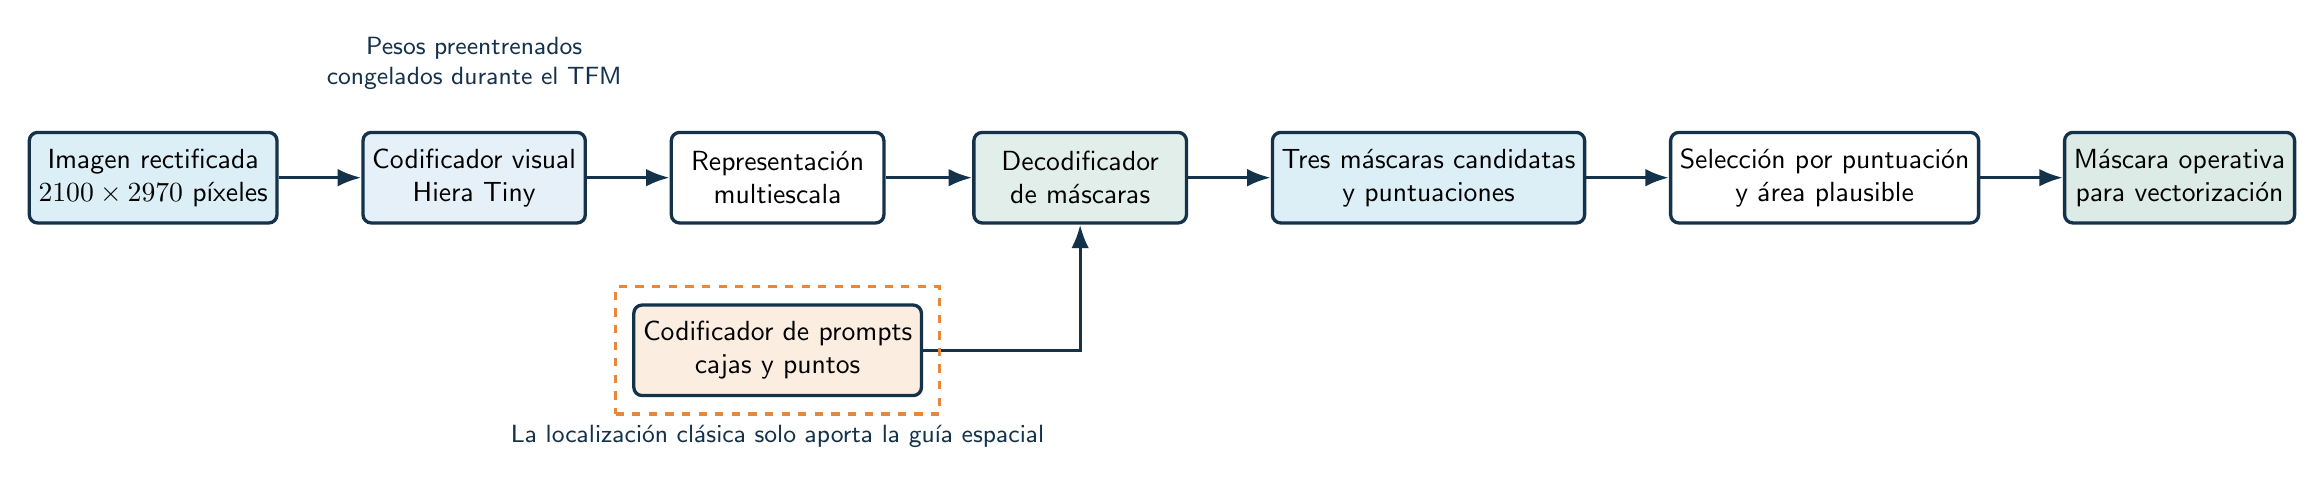
\begin{tikzpicture}[node distance=0.8cm and 1.05cm]
\node[box,fill=cyan] (image) {Imagen rectificada\\$2100\times2970$ píxeles};
\node[box,right=of image,fill=blue!12] (encoder) {Codificador visual\\Hiera Tiny};
\node[box,right=of encoder] (embedding) {Representación\\multiescala};
\node[box,below=1.0cm of embedding,fill=orange!15] (prompt) {Codificador de prompts\\cajas y puntos};
\node[box,right=1.1cm of embedding,fill=green!15] (decoder) {Decodificador\\de máscaras};
\node[box,right=of decoder,fill=cyan] (candidates) {Tres máscaras candidatas\\y puntuaciones};
\node[box,right=of candidates] (selection) {Selección por puntuación\\y área plausible};
\node[box,right=of selection,fill=green!18] (mask) {Máscara operativa\\para vectorización};
\draw[arr] (image)--(encoder); \draw[arr] (encoder)--(embedding); \draw[arr] (embedding)--(decoder);
\draw[arr] (prompt)-|(decoder); \draw[arr] (decoder)--(candidates); \draw[arr] (candidates)--(selection); \draw[arr] (selection)--(mask);
\node[draw=orange,dashed,very thick,fit=(prompt),inner sep=6pt,label={[navy,font=\sffamily\small]below:La localización clásica solo aporta la guía espacial}] {};
\node[navy,font=\sffamily\small,align=center,above=0.4cm of encoder] {Pesos preentrenados\\congelados durante el TFM};
\end{tikzpicture}
\end{document}
